\documentclass[11pt]{beamer}\usepackage[]{graphicx}\usepackage[]{color}
%% maxwidth is the original width if it is less than linewidth
%% otherwise use linewidth (to make sure the graphics do not exceed the margin)
\makeatletter
\def\maxwidth{ %
  \ifdim\Gin@nat@width>\linewidth
    \linewidth
  \else
    \Gin@nat@width
  \fi
}
\makeatother

\definecolor{fgcolor}{rgb}{0.345, 0.345, 0.345}
\newcommand{\hlnum}[1]{\textcolor[rgb]{0.686,0.059,0.569}{#1}}%
\newcommand{\hlstr}[1]{\textcolor[rgb]{0.192,0.494,0.8}{#1}}%
\newcommand{\hlcom}[1]{\textcolor[rgb]{0.678,0.584,0.686}{\textit{#1}}}%
\newcommand{\hlopt}[1]{\textcolor[rgb]{0,0,0}{#1}}%
\newcommand{\hlstd}[1]{\textcolor[rgb]{0.345,0.345,0.345}{#1}}%
\newcommand{\hlkwa}[1]{\textcolor[rgb]{0.161,0.373,0.58}{\textbf{#1}}}%
\newcommand{\hlkwb}[1]{\textcolor[rgb]{0.69,0.353,0.396}{#1}}%
\newcommand{\hlkwc}[1]{\textcolor[rgb]{0.333,0.667,0.333}{#1}}%
\newcommand{\hlkwd}[1]{\textcolor[rgb]{0.737,0.353,0.396}{\textbf{#1}}}%

\usepackage{framed}
\makeatletter
\newenvironment{kframe}{%
 \def\at@end@of@kframe{}%
 \ifinner\ifhmode%
  \def\at@end@of@kframe{\end{minipage}}%
  \begin{minipage}{\columnwidth}%
 \fi\fi%
 \def\FrameCommand##1{\hskip\@totalleftmargin \hskip-\fboxsep
 \colorbox{shadecolor}{##1}\hskip-\fboxsep
     % There is no \\@totalrightmargin, so:
     \hskip-\linewidth \hskip-\@totalleftmargin \hskip\columnwidth}%
 \MakeFramed {\advance\hsize-\width
   \@totalleftmargin\z@ \linewidth\hsize
   \@setminipage}}%
 {\par\unskip\endMakeFramed%
 \at@end@of@kframe}
\makeatother

\definecolor{shadecolor}{rgb}{.97, .97, .97}
\definecolor{messagecolor}{rgb}{0, 0, 0}
\definecolor{warningcolor}{rgb}{1, 0, 1}
\definecolor{errorcolor}{rgb}{1, 0, 0}
\newenvironment{knitrout}{}{} % an empty environment to be redefined in TeX

\usepackage{alltt}
\usetheme{Warsaw}
\usepackage[utf8]{inputenc}
\usepackage{amsmath}
\usepackage{amsfonts}
\usepackage{amssymb}
\usepackage{array}
\usepackage{graphicx}
\author{John Muschelli}
\usepackage{hyperref}
\usepackage{tikz}
\usetikzlibrary{calc,intersections}

\usetikzlibrary{shapes,arrows}
\usetikzlibrary{positioning}
\setbeamertemplate{navigation symbols}{}%remove navigation symbols

\title{Neuroimaging Processing R}
%\setbeamercovered{transparent} 
%\setbeamertemplate{navigation symbols}{} 
%\logo{} 
\institute{Johns Hopkins Bloomberg School of Public Health} 
%\date{} 
%\subject{} 
\setlength{\topsep}{0pt}
\setlength{\parskip}{0pt}
\setlength{\partopsep}{1pt}
\setbeamertemplate{footline}[frame number]

\usepackage[
  natbib = true,
    backend=bibtex,
]{biblatex}
\bibliography{fslr_reg}
\AtEveryBibitem{
\clearfield{note}
% \clearlist{address}
% \clearfield{eprint}
% \clearfield{isbn}
% \clearfield{issn}
% \clearlist{location}
% \clearfield{month}
% \clearfield{series}
} % clears language


\newcommand {\framedgraphic}[2] {
    \begin{frame}{#1}
        \begin{center}
            \includegraphics[width=\textwidth,height=0.8\textheight,keepaspectratio]{#2}
        \end{center}
    \end{frame}
}
\IfFileExists{upquote.sty}{\usepackage{upquote}}{}
\begin{document}

\begin{frame}
\titlepage
\end{frame}

%\begin{frame}
%\tableofcontents
%\end{frame}




\begin{frame}[fragile]{What makes a comprehensive (s)MRI library}

\begin{itemize}

\item Read/Write NIfTI images
\item Visualize Images
\item Inhomogeneity/Bias-field Correction
\item Segmentation
  \begin{itemize}
    \item Brain Extraction
    \item Tissue-Class Segmentation (WM, GM, CSF)
  \end{itemize}
\item Spatial "Normalization"/Registration 
  \begin{itemize}
    \item Within Visit
    \item Across Visit/People
  \end{itemize}
\item Intensity Normalization

\end{itemize}
\end{frame}

\begin{frame}[fragile]{FSL and fslr}

\begin{itemize}
\item FSL is a comprehensive library of analysis tools for fMRI, MRI and DTI brain imaging data. 
  \begin{itemize}
  \item Collection of routines in C, C++
  \end{itemize}
\item fslr: port of FSL into R
\item The two functions we focus on are: 
\begin{enumerate}
\item Brain Extraction Tool (BET)
\item Image inhomogeneity correction and Tissue-class Segmentation (using FAST \citep{zhang2001segmentation})
\end{enumerate} 
\end{itemize}

\end{frame}

\begin{frame}[fragile]{ANTS and ANTsR}

\begin{itemize}
\item Advanced normalization tools (ANTS) \citep{avants2011reproducible} is state-of-the art software that can perform many neuroimaging-related functions.  
  \begin{itemize}
	\item Collection of routines in C, C++, and some R
	\end{itemize}
\item ANTsR: port of ANTS into R using Rcpp
\item The two functions we focus on are: 
\begin{enumerate}
\item Image inhomogeneity correction (N3 \citep{sled1998nonparametric} and N4 \citep{tustison2010n4itk})
\item Tissue-Class Segmentation (Atropos/K-means)
\item Image registration (Symmetric Normalization)
\end{enumerate} 
\end{itemize}

\end{frame}

\begin{frame}[fragile]{extrantsr and WhiteStripe}

\begin{itemize}
\item extrantsr:

{\bf Extr}a {\bf ANTsR} functions.

ANTsR has some non-intuitive syntax and structures.  I created extrantsr to make thing easier and create pipelines. 

\item WhiteStripe:

WhiteStripe from \citet{shinohara2013normalization}:
intensity-based normalization of T1 and T2 image that estimates a white matter mean and standard deviation on data rigidly-registered to the MNI template using histogram-based methods.

\end{itemize}
\end{frame}


\begin{frame}[fragile]{Installing These Packages}
First, you must Install FSL \href{http://fsl.fmrib.ox.ac.uk/fsl/fslwiki/FslInstallation}{http://fsl.fmrib.ox.ac.uk/fsl/fslwiki/FslInstallation}.  \\
\vspace{0.5cm}

\verb|fslr| is installed on CRAN, but the development arm of \verb|fslr| is most likely the best to install, using the \verb|devtools| package (requires new version of \verb|oro.nifti|)

ANTsR is currently (as of April 3, 2015) hosted on GitHub.  

\begin{knitrout}
\definecolor{shadecolor}{rgb}{0.969, 0.969, 0.969}\color{fgcolor}\begin{kframe}
\begin{alltt}
\hlkwa{if} \hlstd{(}\hlopt{!}\hlkwd{require}\hlstd{(devtools))\{}
        \hlkwd{install.packages}\hlstd{(}\hlstr{'devtools'}\hlstd{)}
\hlstd{\}}
\hlstd{devtools}\hlopt{::}\hlkwd{install_github}\hlstd{(}\hlstr{"muschellij2/oro.nifti"}\hlstd{)}
\hlstd{devtools}\hlopt{::}\hlkwd{install_github}\hlstd{(}\hlstr{"muschellij2/fslr"}\hlstd{)}
\hlkwd{install.package}\hlstd{(}\hlstr{"WhiteStripe"}\hlstd{)}
\hlstd{devtools}\hlopt{::}\hlkwd{install_github}\hlstd{(}\hlstr{"stnava/cmaker"}\hlstd{)}
\hlstd{devtools}\hlopt{::}\hlkwd{install_github}\hlstd{(}\hlstr{"stnava/ITKR"}\hlstd{)}
\hlstd{devtools}\hlopt{::}\hlkwd{install_github}\hlstd{(}\hlstr{"stnava/ANTsR"}\hlstd{)}
\end{alltt}
\end{kframe}
\end{knitrout}

\end{frame}

\begin{frame}[fragile]{Installing These Packages}

Setup for JHPCE Cluster is here:

\url{http://muschellij2.github.io/neuro_cluster/README.html
}

\end{frame}



\begin{frame}[fragile]{Unix}

FSL works only on Unix-type machines, so \verb|fslr| only works on Unix-type machines. 

\end{frame}


\begin{frame}[fragile]{Structure of fslr functions}

\tikzstyle{bblock} = [rectangle, draw, text width=7em, text centered, minimum height=2em, rounded corners, align=flush center]
\tikzstyle{line} = [draw, text centered , -latex']
\tikzstyle{line node} = [draw, fill=white, font=\tiny ]
\tikzstyle{block} = [rectangle, draw, text width=5em, text centered, minimum height=4em, rounded corners]

\begin{figure}
\centering
\begin{tikzpicture}[node distance = .5cm, every node/.style={rectangle,fill=white},  transform shape]
% Place nodes
\node [bblock] (fname) {Character filename};
%\node [bblock, right=1cm of fname] (nim) {\verb|nifti| object};
\node [bblock, below right=1cm and 0.1cm of fname] (fslr_func) {fslr function (call FSL function) };
%\node [bblock, above right=1cm and 0.1cm of fslr_func] (nim) {nifti object in R };
\node [bblock, right=3cm of fname] (nim) {nifti object in R };
\node [bblock, below left=1cm and 0.1cm of fslr_func] (nii_back) { Return nifti object to R };
\node [bblock, right=3cm of nii_back] (write) { Write Image to Disk };


% Draw edges
%\path [line] (nim) -| node[xshift=-0.1cm] {} ([xshift=.1 cm]fslr_func.north);
%\path [line] (fname) -| node[xshift=0.1cm] {or} ([xshift=-.1 cm]fslr_func.north);
\path [line] (nim) -| node {} (fslr_func.north);
\path [line] (fname) -| node {or} (fslr_func.north);
%\path [line] (fname) -| ([xshift=-.1 cm]fslr_func.north);
\path [line] ([xshift=.1 cm]fslr_func.south) |- node[xshift=0.1cm] {} (write);
\path [line] ([xshift=-.1 cm]fslr_func.south) |- node[xshift=0.1cm] {and/or} (nii_back);
%\path [line] ([xshift=-.1 cm]fslr_func.south) |- (nii_back);
%\path [line] (fslr_func) |- (write);
%\coordinate[xshift=0.1 cm] (fslr_func) at (write);
%\path [line] (fslr_func) |- (write)+(0,0.1 cm);

\end{tikzpicture}
\end{figure}

\end{frame}




\begin{frame}[fragile]{Reading and Writing Images}
The \verb|oro.nifti| does most of the reading/writing of NIfTI images:

\begin{knitrout}
\definecolor{shadecolor}{rgb}{0.969, 0.969, 0.969}\color{fgcolor}\begin{kframe}
\begin{alltt}
\hlkwd{library}\hlstd{(oro.nifti)}
\hlstd{nim} \hlkwb{=} \hlkwd{readNIfTI}\hlstd{(}\hlstr{"Output_3D_File.nii.gz"}\hlstd{,}
\hlkwc{reorient}\hlstd{=}\hlnum{FALSE}\hlstd{)}
\hlstd{nim}
\end{alltt}
\end{kframe}
\end{knitrout}
\end{frame}

\begin{frame}[fragile]{Reading in Images using ANTsR}
Reading in images using ANTsR requires 2 changes compared to \verb|readNIfTI| from \verb|oro.nifti|:
\begin{enumerate}
\item The extension of the filename (e.g. \verb|.nii.gz|) must be specified
\item The dimension of the image (usually 3) must be supplied (could be 2, 3, or 4)
\end{enumerate}

\begin{knitrout}
\definecolor{shadecolor}{rgb}{0.969, 0.969, 0.969}\color{fgcolor}\begin{kframe}
\begin{alltt}
\hlkwd{library}\hlstd{(ANTsR)}
\hlstd{aimg} \hlkwb{=} \hlkwd{antsImageRead}\hlstd{(}\hlstr{"Output_3D_File.nii.gz"}\hlstd{,}
\hlkwc{dimension} \hlstd{=} \hlnum{3}\hlstd{)}
\end{alltt}
\end{kframe}
\end{knitrout}
\end{frame}

\begin{frame}[fragile]{ANTsR images}

The \verb|aimg| object is an object of \verb|antsImage|, which consists of:
\begin{itemize}
\item pixeltype - how is the image stored (integers versus fractional numbers (floats))
\item dimension - how many dimensions does the image have
\item pointer - where the data is stored
\end{itemize}

\begin{knitrout}
\definecolor{shadecolor}{rgb}{0.969, 0.969, 0.969}\color{fgcolor}\begin{kframe}
\begin{alltt}
\hlkwd{class}\hlstd{(aimg)}
\hlstd{aimg}
\hlkwd{slotNames}\hlstd{(aimg)}
\end{alltt}
\end{kframe}
\end{knitrout}
\end{frame}


\begin{frame}[fragile]{Visualizing Images}

\begin{knitrout}
\definecolor{shadecolor}{rgb}{0.969, 0.969, 0.969}\color{fgcolor}\begin{kframe}
\begin{alltt}
\hlkwd{orthographic}\hlstd{(nim)}
\end{alltt}
\end{kframe}
\end{knitrout}

\end{frame}


\begin{frame}[fragile]{Visualizing Images with an Overlay}
Viewing the image and overlaying in red values $> 200$)
\begin{knitrout}
\definecolor{shadecolor}{rgb}{0.969, 0.969, 0.969}\color{fgcolor}\begin{kframe}
\begin{alltt}
\hlkwd{library}\hlstd{(fslr)}
\hlkwd{ortho2}\hlstd{(nim, nim} \hlopt{>} \hlnum{200}\hlstd{,} \hlkwc{col.y}\hlstd{=}\hlkwd{alpha}\hlstd{(}\hlstr{"red"}\hlstd{,} \hlnum{0.5}\hlstd{))}
\end{alltt}
\end{kframe}
\end{knitrout}

\end{frame}


\begin{frame}[fragile]{Inhomogeneity/Bias-Field Correction}

ANTsR has \verb|n3BiasFieldCorrection| and \verb|n4BiasFieldCorrection|.  These require \verb|antsImage| objects to run.  \\

\vspace{0.5in}
\verb|extrantsr::bias_correct| will perform either of these, you just need to switch \verb|correction|


\begin{knitrout}
\definecolor{shadecolor}{rgb}{0.969, 0.969, 0.969}\color{fgcolor}\begin{kframe}
\begin{alltt}
\hlkwd{library}\hlstd{(extrantsr)}
\hlstd{n4img} \hlkwb{=} \hlkwd{bias_correct}\hlstd{(nim,} \hlkwc{correction} \hlstd{=}\hlstr{"N4"}\hlstd{,} \hlkwc{retimg}\hlstd{=}\hlnum{TRUE}\hlstd{)}
\end{alltt}
\end{kframe}
\end{knitrout}
\end{frame}


\begin{frame}[fragile]{fslr: Brain Extraction}

FSL's Brain Extraction Tool (BET) can be used for skull stripping.  It is fast, robust, and one of the most popular for this task.  \verb|fslr::fslbet| is used to call the FSL commands \verb|bet2|, which does brain extraction or \verb|bet|, which does brain extraction with additional options.



\begin{knitrout}
\definecolor{shadecolor}{rgb}{0.969, 0.969, 0.969}\color{fgcolor}\begin{kframe}
\begin{alltt}
\hlstd{brain_img} \hlkwb{=} \hlkwd{fslbet}\hlstd{(}\hlkwc{infile}\hlstd{=n4img,} \hlkwc{retimg}\hlstd{=}\hlnum{TRUE}\hlstd{)}
\hlcom{### rerurn with new cog}
\hlstd{cog} \hlkwb{=} \hlkwd{cog}\hlstd{(brain_img,} \hlkwc{ceil}\hlstd{=}\hlnum{TRUE}\hlstd{)}
\hlstd{brain_img2} \hlkwb{=} \hlkwd{fslbet}\hlstd{(}\hlkwc{infile}\hlstd{=n4img,}
                    \hlkwc{retimg}\hlstd{=}\hlnum{TRUE}\hlstd{,}
                    \hlkwc{opts} \hlstd{=} \hlkwd{paste}\hlstd{(}\hlstr{"-c"}\hlstd{,} \hlkwd{paste}\hlstd{(cog,} \hlkwc{collapse}\hlstd{=} \hlstr{" "}\hlstd{)))}
\end{alltt}
\end{kframe}
\end{knitrout}
\end{frame}




\begin{frame}[fragile]{fslr: Brain Extraction Results}

\begin{tabular}{ccc}
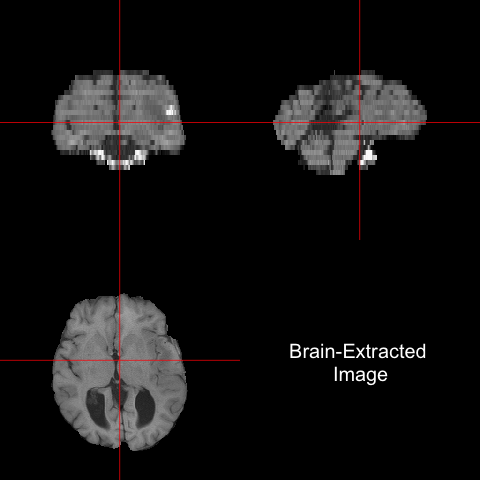
\includegraphics[width=0.32\linewidth]{BET_Image.png} & 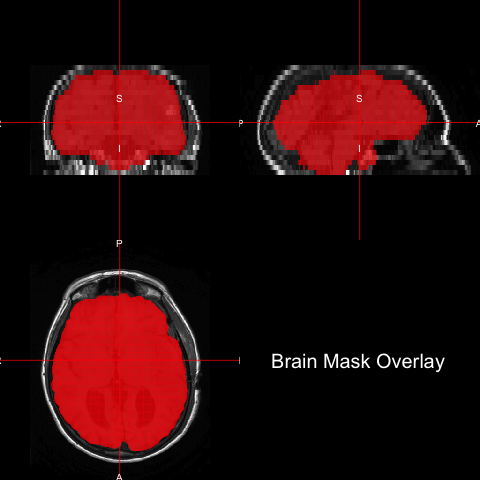
\includegraphics[width=0.32\linewidth]{BET_Image_Overlay.png} & 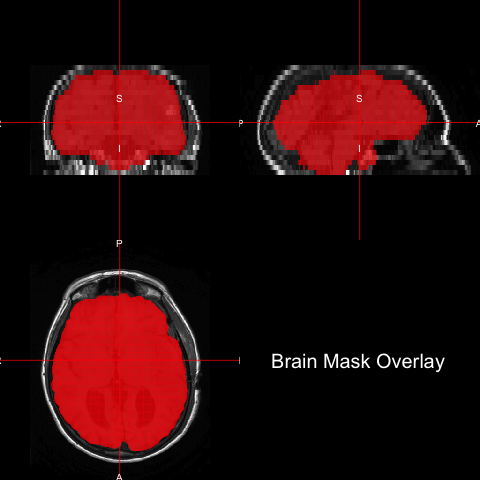
\includegraphics[width=0.32\linewidth]{BET_Image_Overlay.png} 
\end{tabular}

\end{frame}

\begin{frame}[fragile]{ANTsR: Tissue class Segmentation}

Below is some code to do k-means segmentation of an image (k=5) and then finding the one with the highest intensity (white matter). (discuss \verb|ants2oro|)

\begin{knitrout}
\definecolor{shadecolor}{rgb}{0.969, 0.969, 0.969}\color{fgcolor}\begin{kframe}
\begin{alltt}
\hlkwd{library}\hlstd{(fslr)}
\hlstd{a} \hlkwb{=} \hlkwd{oro2ants}\hlstd{(brain_img2)}
\hlstd{x} \hlkwb{=} \hlkwd{oro2ants}\hlstd{((brain_img2}\hlopt{>}\hlnum{0}\hlstd{)}\hlopt{*}\hlnum{1}\hlstd{)}
\hlstd{k} \hlkwb{=} \hlnum{5}\hlstd{; km} \hlkwb{=} \hlkwd{kmeansSegmentation}\hlstd{(a,} \hlkwc{k}\hlstd{=k,} \hlkwc{kmask}\hlstd{=x)}
\hlstd{res} \hlkwb{=} \hlkwd{ants2oro}\hlstd{(km}\hlopt{$}\hlstd{segmentation)}
\hlstd{voxsize} \hlkwb{=} \hlkwd{prod}\hlstd{(}\hlkwd{voxdim}\hlstd{(n4img))}\hlopt{/}\hlnum{1000}
\hlstd{ks} \hlkwb{=} \hlkwd{seq}\hlstd{(k); sizes} \hlkwb{=} \hlkwd{sapply}\hlstd{(ks,} \hlkwa{function}\hlstd{(}\hlkwc{i}\hlstd{)} \hlkwd{sum}\hlstd{(res} \hlopt{==} \hlstd{i))} \hlopt{*} \hlstd{voxsize}
\hlstd{keep_ks} \hlkwb{=} \hlstd{ks[ sizes} \hlopt{>} \hlnum{200} \hlstd{]} \hlcom{# Arbitrary size - need to be "big"}
\hlstd{wm} \hlkwb{=} \hlkwd{cal_img}\hlstd{(res} \hlopt{==} \hlkwd{max}\hlstd{(keep_ks))}
\end{alltt}
\end{kframe}
\end{knitrout}



\end{frame}

\begin{frame}[fragile]{fslr: FAST tissue-class segmentation}



\begin{knitrout}
\definecolor{shadecolor}{rgb}{0.969, 0.969, 0.969}\color{fgcolor}\begin{kframe}
\begin{alltt}
\hlstd{fast_img}  \hlkwb{=} \hlkwd{readNIfTI}\hlstd{(}\hlstr{"test_fast_seg.nii.gz"}\hlstd{,} \hlkwc{reorient}\hlstd{=}\hlnum{FALSE}\hlstd{)}
\end{alltt}
\end{kframe}
\end{knitrout}



\end{frame}

\begin{frame}[fragile]{Tissue-Extraction Results}

\begin{tabular}{cc}
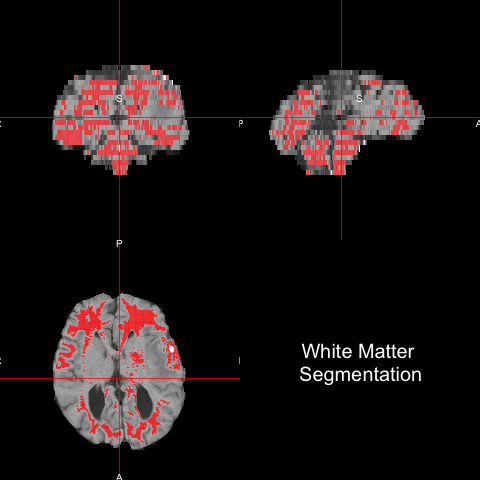
\includegraphics[width=0.5\linewidth]{WM_Image.png} & 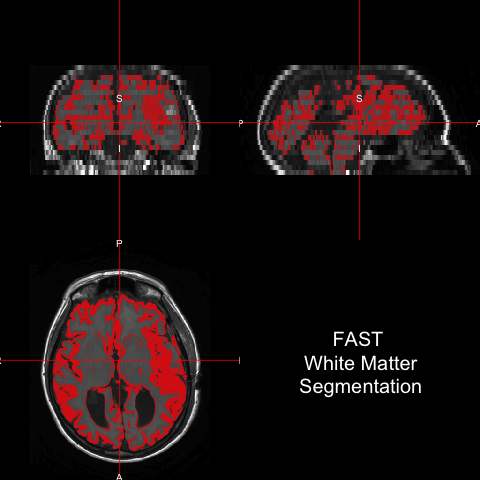
\includegraphics[width=0.5\linewidth]{FAST_Image.png}
\end{tabular}

\end{frame}


\begin{frame}[fragile]{Image Registration}

\begin{itemize}

\item fslr
  \begin{itemize}
  
  \item flirt - linear (rigid/affine) registration
  \item fnirt - non-linear registration
  
  \end{itemize}
  
\item ANTsR: antsRegistration
  \begin{itemize}
  
  \item Rigid/Affine
  \item SyN - symmetric Normalization (REVERSIBLE non-linear registration)
  
  \end{itemize}  

\end{itemize}

\end{frame}


\begin{frame}[fragile]{Image Registration: to Template}

\verb|extrantsr::ants_regwrite| will register images (nifti objects or filenames), write outfiles, 



\begin{knitrout}
\definecolor{shadecolor}{rgb}{0.969, 0.969, 0.969}\color{fgcolor}\begin{kframe}
\begin{alltt}
\hlstd{brain_to_temp} \hlkwb{=} \hlkwd{ants_regwrite}\hlstd{(}\hlkwc{file} \hlstd{= brain_img2,}
                              \hlkwc{template.file} \hlstd{=} \hlstr{"MNI152_T1_1mm_brain.nii.gz"}\hlstd{,}
                              \hlkwc{typeofTransform} \hlstd{=} \hlstr{"SyN"}\hlstd{)}
\end{alltt}
\end{kframe}
\end{knitrout}

\end{frame}




% \begin{frame}[fragile]{Image Registration to Template Results}
% 
% \begin{tabular}{cc}
% 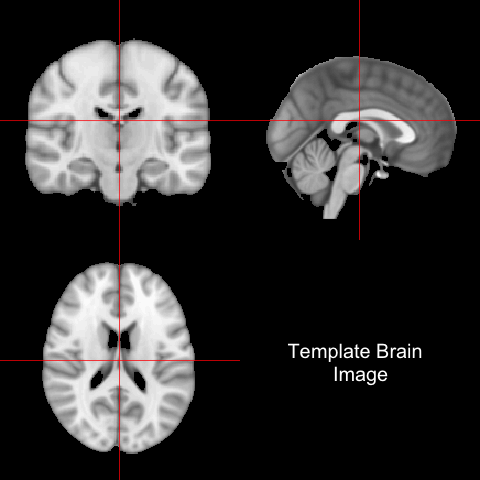
\includegraphics[width=0.5\linewidth]{Template_brain.png} & \includegraphics[width=0.5\linewidth]{SyN_Reg_Image.png}
% \end{tabular}
% 
% \end{frame}


\begin{frame}[fragile]{CRAN/NITRC is not good enough}

\begin{itemize}
\item CRAN is great for R.

\item CRAN is bad for neuroimaging.

\item NITRC is not good enough for neuroimaging (Neuroimaging Informatics Tools and Resources Clearinghouse)

\end{itemize}
\end{frame}


\begin{frame}[fragile]{GitHub has what we need}

\begin{itemize}
\item Version control (obviously)

\item Install packages via \verb|devtools::install_github|

\item Stars for GitHub Packages

\item Travis CI for checking builds

\item Issue pages

\item Data Packages (if github.com)

\item Collaborations

\item Live development version

\end{itemize}

\end{frame}


\begin{frame}[t,allowframebreaks]
  \frametitle{References}
  \printbibliography
 \end{frame}


\begin{frame}[fragile]{Interactive/GUI vs. Terminal R}

In general, GUI-based apps do not inherit the shell environment (aka if \verb|FSLDIR| is defined in your Terminal, RStudio doesn't see it).

For fslr to work, it must know where the directory FSL was installed.  If \verb|FSLDIR| is found, it will be used.  You can check this by 2 ways:

\begin{knitrout}
\definecolor{shadecolor}{rgb}{0.969, 0.969, 0.969}\color{fgcolor}\begin{kframe}
\begin{alltt}
\hlkwd{Sys.getenv}\hlstd{(}\hlstr{"FSLDIR"}\hlstd{)}
\hlkwd{library}\hlstd{(fslr)}
\hlkwd{have.fsl}\hlstd{()}
\end{alltt}
\end{kframe}
\end{knitrout}

If \verb|have.fsl()= FALSE| then you must specify the path using:

\begin{knitrout}
\definecolor{shadecolor}{rgb}{0.969, 0.969, 0.969}\color{fgcolor}\begin{kframe}
\begin{alltt}
\hlkwd{options}\hlstd{(}\hlkwc{fsl.path}\hlstd{=}\hlstr{"/my/path/to/fsl"}\hlstd{)}
\end{alltt}
\end{kframe}
\end{knitrout}


\end{frame}


\begin{frame}[fragile]{Functions of Note}

\verb|extrantsr::preprocess_mri_within| - will N4 (or N3) correct images, co-register scans to the first (T1w usually) scan, skull strip the image (using BET)

\end{frame}


\end{document}
